\documentclass{standalone}
\usepackage{tikz}
\usetikzlibrary{patterns, positioning}


\begin{document}
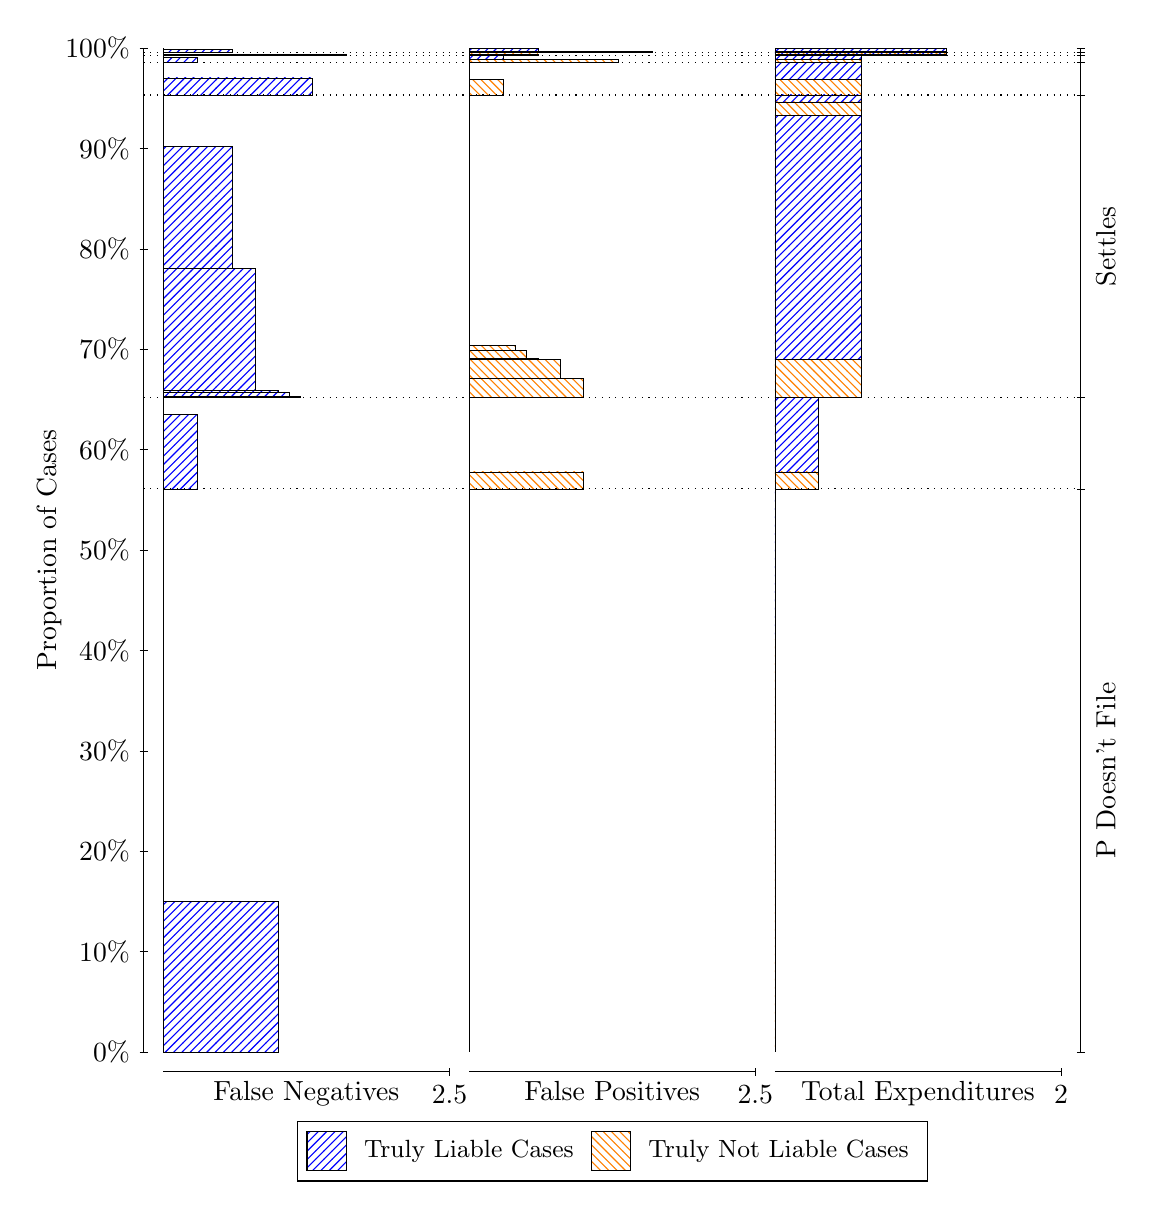
\begin{tikzpicture}
\draw[black, very thin] (1.5,1.75) -- (1.5,14.5);
\node[rotate=90, text=black, anchor=center] at (0.3, 8.125) {Proportion of Cases};
\draw[black, very thin] (1.45,1.75) -- (1.55,1.75);
\node[text=black, anchor=east] at (1.45, 1.75) {0\%};
\draw[black, very thin] (1.45,3.025) -- (1.55,3.025);
\node[text=black, anchor=east] at (1.45, 3.025) {10\%};
\draw[black, very thin] (1.45,4.3) -- (1.55,4.3);
\node[text=black, anchor=east] at (1.45, 4.3) {20\%};
\draw[black, very thin] (1.45,5.575) -- (1.55,5.575);
\node[text=black, anchor=east] at (1.45, 5.575) {30\%};
\draw[black, very thin] (1.45,6.85) -- (1.55,6.85);
\node[text=black, anchor=east] at (1.45, 6.85) {40\%};
\draw[black, very thin] (1.45,8.125) -- (1.55,8.125);
\node[text=black, anchor=east] at (1.45, 8.125) {50\%};
\draw[black, very thin] (1.45,9.4) -- (1.55,9.4);
\node[text=black, anchor=east] at (1.45, 9.4) {60\%};
\draw[black, very thin] (1.45,10.675) -- (1.55,10.675);
\node[text=black, anchor=east] at (1.45, 10.675) {70\%};
\draw[black, very thin] (1.45,11.95) -- (1.55,11.95);
\node[text=black, anchor=east] at (1.45, 11.95) {80\%};
\draw[black, very thin] (1.45,13.225) -- (1.55,13.225);
\node[text=black, anchor=east] at (1.45, 13.225) {90\%};
\draw[black, very thin] (1.45,14.5) -- (1.55,14.5);
\node[text=black, anchor=east] at (1.45, 14.5) {100\%};

\draw[black, very thin] (13.4,1.75) -- (13.4,14.5);
\draw[black, very thin] (13.35,1.75) -- (13.45,1.75);
\node[anchor=west] at (13.35, 1.75) {};
\draw[black, very thin] (13.35,8.9019) -- (13.45,8.9019);
\node[anchor=west] at (13.35, 8.9019) {};
\draw[black, very thin] (13.35,10.063) -- (13.45,10.063);
\node[anchor=west] at (13.35, 10.063) {};
\draw[black, very thin] (13.35,13.904) -- (13.45,13.904);
\node[anchor=west] at (13.35, 13.904) {};
\draw[black, very thin] (13.35,14.321) -- (13.45,14.321);
\node[anchor=west] at (13.35, 14.321) {};
\draw[black, very thin] (13.35,14.409) -- (13.45,14.409);
\node[anchor=west] at (13.35, 14.409) {};
\draw[black, very thin] (13.35,14.44) -- (13.45,14.44);
\node[anchor=west] at (13.35, 14.44) {};
\draw[black, very thin] (13.35,14.5) -- (13.45,14.5);
\node[anchor=west] at (13.35, 14.5) {};

\draw[black, very thin, pattern color=blue, pattern=north east lines] (1.75,1.75) rectangle (3.2033,3.6602);
\draw[black, very thin, pattern color=orange, pattern=north west lines] (1.75,3.6602) rectangle (1.75,8.9019);
\draw[black, very thin, pattern color=blue, pattern=north east lines] (1.75,8.9019) rectangle (2.186,9.8493);
\draw[black, very thin, pattern color=orange, pattern=north west lines] (1.75,9.8493) rectangle (1.75,10.063);
\draw[black, very thin, pattern color=blue, pattern=north east lines] (1.75,10.063) rectangle (3.494,10.076);
\draw[black, very thin, pattern color=blue, pattern=north east lines] (1.75,10.076) rectangle (3.3487,10.131);
\draw[black, very thin, pattern color=blue, pattern=north east lines] (1.75,10.131) rectangle (3.2033,10.152);
\draw[black, very thin, pattern color=blue, pattern=north east lines] (1.75,10.152) rectangle (2.9127,11.7);
\draw[black, very thin, pattern color=blue, pattern=north east lines] (1.75,11.7) rectangle (2.622,13.248);
\draw[black, very thin, pattern color=orange, pattern=north west lines] (1.75,13.248) rectangle (1.75,13.904);
\draw[black, very thin, pattern color=blue, pattern=north east lines] (1.75,13.904) rectangle (3.6393,14.12);
\draw[black, very thin, pattern color=orange, pattern=north west lines] (1.75,14.12) rectangle (1.75,14.321);
\draw[black, very thin, pattern color=blue, pattern=north east lines] (1.75,14.321) rectangle (2.186,14.378);
\draw[black, very thin, pattern color=orange, pattern=north west lines] (1.75,14.378) rectangle (1.75,14.409);
\draw[black, very thin, pattern color=blue, pattern=north east lines] (1.75,14.409) rectangle (4.0753,14.423);
\draw[black, very thin, pattern color=orange, pattern=north west lines] (1.75,14.423) rectangle (1.75,14.44);
\draw[black, very thin, pattern color=blue, pattern=north east lines] (1.75,14.44) rectangle (2.622,14.486);
\draw[black, very thin, pattern color=orange, pattern=north west lines] (1.75,14.486) rectangle (1.75,14.5);
\draw[black, very thin, pattern color=orange, pattern=north west lines] (5.6333,1.75) rectangle (5.6333,6.9917);
\draw[black, very thin, pattern color=blue, pattern=north east lines] (5.6333,6.9917) rectangle (5.6333,8.9019);
\draw[black, very thin, pattern color=orange, pattern=north west lines] (5.6333,8.9019) rectangle (7.0867,9.1159);
\draw[black, very thin, pattern color=blue, pattern=north east lines] (5.6333,9.1159) rectangle (5.6333,10.063);
\draw[black, very thin, pattern color=orange, pattern=north west lines] (5.6333,10.063) rectangle (7.0867,10.304);
\draw[black, very thin, pattern color=orange, pattern=north west lines] (5.6333,10.304) rectangle (6.796,10.544);
\draw[black, very thin, pattern color=orange, pattern=north west lines] (5.6333,10.544) rectangle (6.5053,10.56);
\draw[black, very thin, pattern color=orange, pattern=north west lines] (5.6333,10.56) rectangle (6.36,10.66);
\draw[black, very thin, pattern color=orange, pattern=north west lines] (5.6333,10.66) rectangle (6.2147,10.719);
\draw[black, very thin, pattern color=blue, pattern=north east lines] (5.6333,10.719) rectangle (5.6333,13.904);
\draw[black, very thin, pattern color=orange, pattern=north west lines] (5.6333,13.904) rectangle (6.0693,14.105);
\draw[black, very thin, pattern color=blue, pattern=north east lines] (5.6333,14.105) rectangle (5.6333,14.321);
\draw[black, very thin, pattern color=orange, pattern=north west lines] (5.6333,14.321) rectangle (7.5227,14.352);
\draw[black, very thin, pattern color=blue, pattern=north east lines] (5.6333,14.352) rectangle (6.0693,14.409);
\draw[black, very thin, pattern color=orange, pattern=north west lines] (5.6333,14.409) rectangle (6.5053,14.426);
\draw[black, very thin, pattern color=blue, pattern=north east lines] (5.6333,14.426) rectangle (5.6333,14.44);
\draw[black, very thin, pattern color=orange, pattern=north west lines] (5.6333,14.44) rectangle (7.9587,14.454);
\draw[black, very thin, pattern color=blue, pattern=north east lines] (5.6333,14.454) rectangle (6.5053,14.5);
\draw[black, very thin, pattern color=orange, pattern=north west lines] (9.5167,1.75) rectangle (9.5167,6.9917);
\draw[black, very thin, pattern color=blue, pattern=north east lines] (9.5167,6.9917) rectangle (9.5167,8.9019);
\draw[black, very thin, pattern color=orange, pattern=north west lines] (9.5167,8.9019) rectangle (10.062,9.1159);
\draw[black, very thin, pattern color=blue, pattern=north east lines] (9.5167,9.1159) rectangle (10.062,10.063);
\draw[black, very thin, pattern color=orange, pattern=north west lines] (9.5167,10.063) rectangle (10.607,10.544);
\draw[black, very thin, pattern color=blue, pattern=north east lines] (9.5167,10.544) rectangle (10.607,13.641);
\draw[black, very thin, pattern color=orange, pattern=north west lines] (9.5167,13.641) rectangle (10.607,13.815);
\draw[black, very thin, pattern color=blue, pattern=north east lines] (9.5167,13.815) rectangle (10.607,13.904);
\draw[black, very thin, pattern color=orange, pattern=north west lines] (9.5167,13.904) rectangle (10.607,14.105);
\draw[black, very thin, pattern color=blue, pattern=north east lines] (9.5167,14.105) rectangle (10.607,14.321);
\draw[black, very thin, pattern color=orange, pattern=north west lines] (9.5167,14.321) rectangle (10.607,14.352);
\draw[black, very thin, pattern color=blue, pattern=north east lines] (9.5167,14.352) rectangle (10.607,14.409);
\draw[black, very thin, pattern color=orange, pattern=north west lines] (9.5167,14.409) rectangle (11.697,14.426);
\draw[black, very thin, pattern color=blue, pattern=north east lines] (9.5167,14.426) rectangle (11.697,14.44);
\draw[black, very thin, pattern color=orange, pattern=north west lines] (9.5167,14.44) rectangle (11.697,14.454);
\draw[black, very thin, pattern color=blue, pattern=north east lines] (9.5167,14.454) rectangle (11.697,14.5);
\draw[black, dotted] (1.5,8.9019) -- (13.4,8.9019);
\draw[black, dotted] (1.5,10.063) -- (13.4,10.063);
\draw[black, dotted] (1.5,13.904) -- (13.4,13.904);
\draw[black, dotted] (1.5,14.321) -- (13.4,14.321);
\draw[black, dotted] (1.5,14.409) -- (13.4,14.409);
\draw[black, dotted] (1.5,14.44) -- (13.4,14.44);
\draw[black, very thin] (1.75,1.5) -- (5.3833,1.5);
\node[text=black, anchor=north] at (3.5667, 1.5) {False Negatives};
\draw[black, very thin] (5.3833,1.45) -- (5.3833,1.55);
\node[text=black, anchor=north] at (5.3833, 1.45) {2.5};

\draw[black, very thin] (5.6333,1.5) -- (9.2667,1.5);
\node[text=black, anchor=north] at (7.45, 1.5) {False Positives};
\draw[black, very thin] (9.2667,1.45) -- (9.2667,1.55);
\node[text=black, anchor=north] at (9.2667, 1.45) {2.5};

\draw[black, very thin] (9.5167,1.5) -- (13.15,1.5);
\node[text=black, anchor=north] at (11.333, 1.5) {Total Expenditures};
\draw[black, very thin] (13.15,1.45) -- (13.15,1.55);
\node[text=black, anchor=north] at (13.15, 1.45) {2};

\node[text=black, centered, rotate=90] at (13.72, 5.3259) {P Doesn't File};

\node[text=black, centered, rotate=90] at (13.72, 11.984) {Settles};





\draw (7.449999999999999,1.5) node[draw=none] (baseCoordinate) {};
\begin{scope}[align=center]
        \matrix[scale=0.5, draw=black, below=0.5cm of baseCoordinate, nodes={draw}, column sep=0.1cm]{
            \node[rectangle, draw, minimum width=0.5cm, minimum height=0.5cm, pattern color=blue, pattern=north east lines] {}; &
            \node[draw=none, font=\small, text=black] (B) {Truly Liable Cases}; &
            \node[rectangle, draw, minimum width=0.5cm, minimum height=0.5cm, pattern color=orange, pattern=north west lines] {}; &
            \node[draw=none, font=\small, text=black] (B) {Truly Not Liable Cases}; \\
            };
\end{scope}

\end{tikzpicture}
\end{document}